%Vorlage fuer Thesen an der FFHS
\documentclass{../template/ffhsthesis}

\usepackage[utf8]{inputenc}

% addional configuration from sam
\usepackage{bibgerm}
\usepackage{hyperref}
\usepackage{cite}
\usepackage{etoolbox}
\usepackage{listings}
\usepackage{wrapfig}
\usepackage{fullpage}
\usepackage[section]{placeins}
\usepackage{float}%
\usepackage{verbatim}
\usepackage{filecontents}
\usepackage{siunitx}
\sisetup{per=slash, load=abbr}
\usepackage{tikz}
\usepackage{pgfplots}
\pgfplotsset{width=7cm,compat=newest}

\makeatother
\hypersetup{
    colorlinks = false,
    linkcolor = blue,
    urlcolor  = blue,
    citecolor = blue,
    anchorcolor = blue,
    pdfborder={0 0 0},
}
\setlength\parindent{0pt}




\begin{document}
% addional configuration from sam
\shorthandoff{"}
\lstdefinelanguage{C}
{
                basicstyle=\ttfamily\small,
                keywordstyle=\color{blue}\ttfamily,
                stringstyle=\color{red}\ttfamily,
                commentstyle=\color{green}\ttfamily,
                morecomment=[l][\color{magenta}]{\#}
}

\lstdefinelanguage
   [x64]{Assembler}     % add a "x64" dialect of Assembler
   [x86masm]{Assembler} % based on the "x86masm" dialect
   % with these extra keywords:
   {morekeywords={CDQE,CQO,CMPSQ,CMPXCHG16B,JRCXZ,LODSQ,MOVSXD, %
                  POPFQ,PUSHFQ,SCASQ,STOSQ,IRETQ,RDTSCP,SWAPGS, %
                  rax,rdx,rcx,rbx,rsi,rdi,rsp,rbp, %
                  r8,r8d,r8w,r8b,r9,r9d,r9w,r9b}} % etc.

\lstset{language=[x64]Assembler}


\lstdefinelanguage{Ini}
{
    basicstyle=\ttfamily\small,
    columns=fullflexible,
    morecomment=[s][\color{blue}\bfseries]{[}{]},
    morecomment=[l]{\#},
    morecomment=[l]{;},
    commentstyle=\color{gray}\ttfamily,
    morekeywords={},
    otherkeywords={=,:},
    keywordstyle={\color{green}\bfseries}
}

% https://github.com/zemirco/tu-darmstadt-latex-thesis


% Farbpalette A
\definecolor{blau_1a}{RGB}{93,133,195}
\definecolor{blau_2a}{RGB}{0,156,218}
\definecolor{gruen_3a}{RGB}{80,182,149}
\definecolor{gruen_4a}{RGB}{175,204,80}
\definecolor{gruen_5a}{RGB}{221,223,72}
\definecolor{orange_6a}{RGB}{255,224,92}
\definecolor{orange_7a}{RGB}{248,186,60}
\definecolor{rot_8a}{RGB}{238,122,52}
\definecolor{rot_9a}{RGB}{233,80,62}
\definecolor{lila_10a}{RGB}{201,48,142}
\definecolor{lila_11a}{RGB}{128,69,151}

% Farbpalette B
\definecolor{blau_1b}{RGB}{0,90,169}
\definecolor{blau_2b}{RGB}{0,131,204}
\definecolor{gruen_3b}{RGB}{0,157,129}
\definecolor{gruen_4b}{RGB}{153,192,0}
\definecolor{gruen_5b}{RGB}{201,212,0}
\definecolor{orange_6b}{RGB}{253,202,0}
\definecolor{orange_7b}{RGB}{245,163,0}
\definecolor{rot_8b}{RGB}{236,101,0}
\definecolor{rot_9b}{RGB}{230,0,26}
\definecolor{lila_10b}{RGB}{166,0,132}
\definecolor{lila_11b}{RGB}{114,16,133}


\dokumentTyp{Bachelor-Thesis}
\studiengang{INF}
\title{Energie in der Informatik}
\subtitle{ durch bessere Software sparen ohne Verzicht} % optional
\titelbild[height=4.55cm,width=15cm]{images/Italy_Alps_and_Mediterranean.jpg}  % optional
\author{Samuel Riolo}
% \date{}
\wohnort{Kerzers}
%\referent{Name des Referenten\\ Titel\\Unterrichtetes Fach}
\referent{Jürg Hofer\\Dipl. El. Ing. ETH\\WING}
%\referent{Jürg Hofer\\ Titel\\Unterrichtetes Fach}
%\eingereichtBei{Prof.\ Dr.\ Martin Sutter\\Departement Informatik\\Departementsleiter} 


\maketitle

\begin{zusammenfassung}

Die Energiepolitik ist auf der ganzen Welt ein grosses Thema und wird heftig diskutiert. Diese Arbeit befasst sich mit der Zielsetzung, den Energieverbrauch zu senken. Es wird eine Messmethode erforscht und entwickelt, um den Strombedarf eines CPU-Prozessors zu untersuchen. Damit wird dessen Energiebedarf pro Befehlssatz gemessen und analysiert. Dabei hat sich herausgestellt, das eine Verallgemeinerung von Energieverschwenderische Befehlssätze sehr schwer zu erstellen ist, im Gegenzug sollte punktuell eine bestimmte stelle optimiert werden. Die gemessene Differenzen zwischen den Befehlssätze sind von unterschiedlichen Faktoren abhängig, dazu gehört die CPU-Architektur oder die Wortlänge des Operand das berechnet wird. Es wurde gezeigt, dass die grösste Energieeinsparung durch Befehlssätze mit geringeren CPU-Zyklen erreicht wird. 





\end{zusammenfassung}

\begin{abstract} 

-- Just an dirty Google translation as placeholder, I will fix it later --
\par
Energy policy is a big issue around the world and is hotly debated. More and more people are the
Believes that energy policy is unumgäglich. One of the main criteria of the energy transition, however, the
Energy is saved. This work will focus on a subsection of the energy transition. It should be pointed out,
where is the IT industry, especially in the client and server area, potential to save power. economic aspects
should be considered by the success in efficiency, without sacrificing the quality of the IT infrastructure
can be achieved.
\par
The work focused on it, the energy consumption per instruction set of a processor
analyze. It will be researched and developed a measurement methods to examine the current.....

\end{abstract}



\tableofcontents

\begin{abkuerzungen}[MUSTER] % Das Muster dient zur Bestimmung der Einrueckungstiefe
%\item[DInf] Departement Informatik
%\item[FFHS] Fernfachhochschule Schweiz
\item[ALU] Arithmetic Logic Unit
\item[ARM] Advanced RISC Machine
\item[ASCII] American Standard Code for Information Interchange
\item[CISC] Custom Instruction Set Computer
\item[CPU] Central Processing Unit
\item[CU] Control Unit
\item[EpI] Energy per Instruction
\item[GCC] GNU Compiler Collection
\item[GPIO] General-purpose input/output
\item[IRQ] Interrupts Request
\item[ISR] Interrupt-Service-Routine
\item[PCI] Peripheral Component Interconnect
\item[POSIX] Portable Operating System Interface
\item[RAM] Random Access Memory
\item[RISC] Reduced Instruction Set Computer
\item[SoC] System on Chip
\item[TWh/a] $10^{12}$ Wattstunden oder $10^{9}$ Kilowattstunden pro Jahr


\end{abkuerzungen}


\startThesis % Befehl muss vor dem ersten chapter stehen (Seitennummerierung!)


% addional configuration from sam
\addtolength{\parskip}{\baselineskip}
\parindent 0pt 



% content
\chapter{Einleitung}


In der heutigen Zeit ist die nachhaltige Produktion von Energie und ein schonender Umgang mit dieser Ressource ein wichtiges Anliegen der Öffentlichkeit. Der Bundesrat hat einen Teil der Ziele seiner Energiepolitik in dem Partnerschaftsprogramm EnergieSchweiz festgelegt. Aus Sicht der Informatikbranche ist es interessant zu evaluieren, welchen Anteil sie zur Energieeinsparung beitragen kann. Aus der heutigen Gesellschaft sind Computer nicht mehr wegzudenken. Sie sind sowohl im privaten wie im geschäftlichen Bereich weit verbreitet und erleben nach wie vor einen starken Zuwachs. Daher ergibt auch die kleinste Einsparung pro Computer in der Summe ein immenses Energiesparpotenzial und einen beachtlichen quantitativen Anteil am gesamthaften Sparpotenzial. 
\par
In der IT-Branche existieren bereits heute zahlreiche Möglichkeiten, mit welchen ein nachhaltiger und schonender Umgang mit elektrischer Energie erreicht werden kann. Aus allen möglichen Massnahmen zur Energieeinsparung in der Computerwelt wurde hier jene ausgewählt und erforscht, die auf bereits bestehender Hardware umgesetzt werden kann und somit keinen Ersatz dieser erfordert. Die Basis aller Computertätigkeiten ist die Abarbeitung von unendlich vielen Befehlssätzen durch den Prozessor. Selbst Programme, die interpretiert werden oder in einer höheren Programmiersprachen geschrieben wurden, werden schliesslich als eine Reihe von Befehlssätzen auf dem Prozessor ausgeführt. Aus diesem Grundwissen wird folgende Forschungsfrage formuliert: Ist es möglich, durch effizientere Befehlssätze Energie zu sparen?
\par
Um diese Frage zu beantworten, wurde im Rahmen dieser Engineeringarbeit eine Messmethodik zur Analyse des Energiebedarfs eines Prozessors pro Befehlssatz entwickelt. Sie ermöglicht es, den Energiebedarf einzelner, beliebiger Befehlssätze effizient zu messen. So können Daten erstellt, die Informationen über den Energieverbrauch einzelner Befehlssätze liefern. Die Messungen erfolgen dabei auf unterschiedlichen CPU-Architekturen, damit abweichende Messresultate beobachtet werden können.
\par
Im Endeffekt ist das Hauptziel der vorgenommenen Messungen die Evaluation des Energiesparpotentials. Mit dieser Arbeit soll aufgezeigt werden, ob im Softwarebereich Energie gespart werden kann. Gleichzeitig sollen die Messmethodik und die daraus gewonnenen Erkenntnisse als Grundlage für weitergehende Forschungen dienen. So könnten diese beispielsweise zur Optimierung von Smartphones im Sinne einer längeren Akkulaufzeit eingesetzt werden.
\par
Um die technische Aspekte für den Leser nachvollziehbar zu gestalten, wurde mit viele Grafiken gearbeitet. Alle Abbildungen in dieser Arbeit wurden vom Autor selbst erstellt \footnote{Ausgenommen die Produktbilder in den Abbildungen \ref{fig:Intel Galileo Gen2} und \ref{fig:Raspberry Pi 1 A}.}. 












\begin{comment}

In der heutigen Zeit ist die nachhaltige Produktion von Energie und ein schonender Umgang mit dieser Ressource ein wichtiges Anliegen der Öffentlichkeit. Speziell die IT-Branche ist von einem grossen Wachstum geprägt. Immer mehr Tätigkeiten werden automatisiert und bestehende Systeme ausgebaut. Dies verursacht einen immer grösseren Stromverbrauch im IT-Bereich. Ein Ziel der Energiepolitik 2050 ist die Senkung des immer weiter steigenden Energieverbrauchs.
\par
Um in der IT-Branche Energie zu sparen, können verschiedene Ansätze gewählt werden. Beispielsweise besteht die Möglichkeit bei Inaktivität automatisch in den Ruhemodus zu wechseln oder die Prozessoren durch sogenannte Sparmodi, insbesondere dynamische Taktfrequenzen oder das kurzzeitige Ein- und Ausschalten der Rechnereinheit, zu optimieren. Diese Sparansätze zielen jeweils nur auf den Hard- oder Softwarebereich ab. Sie berücksichtigen jedoch nicht die besondere Funktionsweise eines jeden Computers, wo die Software die Hardware, also ein Programm einen Prozessor, ansteuert. Anders im Rahmen dieser Arbeit, in welcher das Sparpotenzial bereichsübergreifend erforscht wird.



\section{Übersicht}

Die Energiepolitik ist auf der ganzen Welt ein grosses Thema und wird heftig diskutiert. Immer mehr Leute
sind der Überzeugung, dass eine Energiewende unumgänglich ist. Dabei wird die Energiewende von politischen, aber auch
von wirtschaftlichen Interessen beeinflusst. Die Energiewende beinhaltet aber nicht nur
das Produzieren von erneuerbaren Energien, sondern viele unterschiedliche Teilaspekte. Für die Energiewende
müssen Energieressourcen gespeichert werden, damit sie bei Bedarf genutzt werden können. Wird Strom über
Solaaranlagen in den Haushalten produziert, so muss die Energie ins Netz zurückfliessen. Dafür müssen
Hochspannungsleitungen so verändert werden, dass sie Strom in beide Richtungen fliessen lassen können.
Die heute verwendeten Energienanlagen, wie Windmühlen oder Solaaranlagen, produzieren in Europa so starke
Schwankungen, dass die Gefahr eines riesigen Blackouts besteht.
\par
Viele Probleme müssen für die Energiewende gelöst werden. Eines der wichtigsten Kriterien der Energiewende ist aber,
dass Energie gespart wird. Diese Arbeit wird sich mit einem Teilgebiet der Energiewende befassen.
Es soll aufgezeigt werden, wo in der IT-Branche, speziell im Client- und Serverbereich, Potenzial besteht,
Strom zu sparen. 

% todo Überarbeiten, ausführlicher
Auch gerade deswegen, weil die IT-Branche von einem enormen Wachstum geprägt ist. Wirtschaftliche Aspekte sollen
berücksichtigt werden, indem der Erfolg des Stromsparens ohne Verzicht auf die Qualität der IT-Infrastruktur erzielt
werden kann. 
\par
% todo Zusammenfassung der Arbeit, nicht Beschreibung, was ich machen werde
Ein Computer ist ein Gerät, dessen Besonderheit darin besteht, dass es durch logische und arithmetische Befehle programmiert
werden kann. In andere Worte gefasst, heisst das, dass die Software die Hardware ansteuert und die Hardware Befehl um Befehl ausführt.
Genau dieser Aspekt soll in der Arbeit abgehandelt werden. Es soll eine Basis gebildet werden, die aufzeigt, wie man durch bessere Software Strom
sparen kann. Die Arbeit wird sich darauf konzentrieren, den Energiebedarf pro Befehlssatz eines Prozessors zu analysieren.
Es soll eine Messmethoden erforscht und entwickelt werden, um den Strombedarf eines CPU zu untersuchen. Die Untersuchung soll
auf unterschiedlichen SoC (System on Chip) Architekturen erfolgen, damit Vergleiche erstellt werden können.
\par
Ziel der Arbeit ist es, Daten zu erhalten, die Informationen über den Energieverbrauch einzelner Befehlssätze liefern. Diese Daten
könnte man zum Beispiel auf Workstations oder Server hochrechnen. Für CPU-Befehle, die sich eher verschwenderisch auf den
Strombedarf auswirken, könnte man Alternativen finden.

\end{comment}


% Denn nur so kann eine Aussage gemacht werden, ob ein neues System auch zielführend ist. Erst im zweiten Schritt können dann
% Ansätze evaluiert werden, die zum Ziel der Reduktion des Energieverbrauchs dienen können. 
% Dabei sollen unterschiedliche Schichten der Software analysiert werden. Es sollen Antworten auf die folgenden Fragen gefunden werden:
% Wie kann das Betriebsystem Strom sparen; ist es möglich durch bessere Treiber die Hardware auf Standby zu setzen, wenn sie nicht gebraucht wird
% oder kann bereits beim Kompilieren effizenter gearbeitet werden. Am Schluss soll geprüft werden,
% ob die Ansätze in der Realität anwendbar und wirtschaflich interessant sind. Es sollen konkrete Beispiele enstehen, wo und wie ein
% IT-Betrieb Stromersparnisse erzielen kann.




\chapter{Energiepolitik 2050}

\section{Energiepolitische Entscheidungen in der Schweiz}
Durch den Beschluss am 2011 des Bundesrat und Parlament wurde ein Grundsatzentscheid getroffen,
schrittweise aus der Kernenergie auszusteigen\cite{bfe_energiestrategie}. 
\par
Die Stillegung der fünf Kernkraftwerke in der Schweiz, sollen am Ende ihrer sicherheitstechnischen
Betriebsdauer erfolgen. Diese Entscheidung und insbesondere auch die internationale Veränderungen 
im der Energieversorgung bewirkt eine starke Wende in das schweizerische Energieumfeld.
Am 4. September 2013 wurde vom Bundesrat und Parlament das erste Massnahmenpaket verabschiedet, um
die Sicherheit der Energieversorgung in der Schweiz zu garantieren. Das Massnahmenpaket setzt in erster
Line auf eine ausgewogene Ausschöpfung der vorhandene Potenziale der Wasserkraft und der neuen erneuerbaren
Energien. Am 8. Dezember 2014 wurde das Massnahmenpaket vom Nationalrat und am 23. September 2015 vom Ständerat
angenommen. Differenzen werden zur Zeit zwischen den Räten bereinigt bevor diese nochmals über die
gesamte Vorlage abstimmt. 
\par
Das Parlament hat bereits mit einer Gesetzesänderung (pa.lv. 12.400) verabschiedet, dass am Anfang 2014 in
Kraft getreten ist. Dadurch werden der Ausbau der erneuerbaren Energien gefördert. Auch beinhaltet
diese Gesetzesänderung ein Aktionsplan für eine stärkere Energieforschung.

\section{Stromnachfrage 2010 - 2050}

Die Prognosen der Stromnachfrage über ein Zeithorizont von 40 Jahren ist generell sehr schwer\cite{eth_energiezukunft_schweiz}.
Dennoch bilden sich plausible Wert für das Jahr 2050 ab. Dabei werden die Parameter Bevölkerungswachstum,
Pro-Kopf-Einkommen und Stromintensität aufgrund der Trends, berücksichtigt.
\par
Heute geht man von einem Stromverbrauch von 63 TWh pro Jahr aus (inkl. Netzverluste von etwa 7\% aber
ohne Speicherpumpenverluste). Für das Jahr 2050 geht man davon aus, dass sich die Extremwerte von
60 TWh/a bis über 100TWh/a abzeichnen werden.
\par
Der schrittweise Ausstieg aus der Atomkraft und gleichzeitig die neuen Ansprüche des Strombedarfs abzudecken,
scheint für das 2050 schwierig aber nicht unmöglich zu sein. Die Transformation des Energiesystem in einem
Zeithorizont von mehrere Jahrzehnten ist im Grundsatz technologisch machbar und wirtschaftlich verkraftbar.
Für den Erfolg muss in die Forschung und Einsatz von Photovoltaik, Biomasse, Wind und Geothermie investiert werden.
Auch der Ausbau von Stauseen, als Pumpspeicherkraftwerken wird dafür nötig sein.
\par
Die CO\textsubscript{2}-Reduzierung und die damit kombinierte Stromerzeugung aus erneuerbare Energien, führt auch dazu,
dass die importiert mengen um 65\% reduziert werden. Dabei wird ein wesentlicher Beitrag geleistet, dass die Schweiz
hinsichtlich der Stromversorgung unabhängiger wird und eine besser  Versorgungssicherheit des Landes gewährleistet wird.
 



\section{}








\chapter{Stand des Wissens und der Technik}
Für den Grundaufbau der Messmethodik ist das Grundwissen über einzelne Elemente unverzichtbar. In diesem Kapitel wird auf spezifisch ausgewählte Punkte eingegangen, um das Verständnis weiterer Zusammenhänge für den Leser zu vereinfachen.


\section{Funktionsweise eines Prozessors}

Ein Prozessor ist eine universelle Rechenmaschine, die sich durch eine definierte Reihe von Anweisungen programmieren lässt. Zu den arithmetischen Anweisungen gehören der Zugriff auf Speicheradressen und Sprünge innerhalb der Abfolge der Anweisungen.
Bereits der britische Mathematiker Alan Turing konnte aufzeigen, dass ein universelles Berechnungsmodell umsetzbar ist, wenn ein Rechner neben dem Speicherzugriff auch Sprünge besitzt\cite{Hoffmann2014l}. Auf diesen besonderen Eigenschaften bauen die heutigen Prozessoren auf. Ein Programm, das den Prozessor ansteuert, besteht aus einer endlichen Anzahl von geordneten Anweisungen. Der Prozessor befolgt, streng nach dem Ablauf, Anweisung für Anweisung. Diese ablaufenden Anweisungen können dabei auch Sprünge zu anderen Stellen innerhalb des Programms definieren.
\par
Die Prozessoren, auch Zentraleinheiten oder CPUs genannt, besitzen im Inneren drei Einheiten, die über einen Datenbus verbunden sind. Dies ist in der \autoref{fig:CPU} ersichtlich. Dabei kann der Datenbus je nach Grösse oder Leistung der CPU variieren. Die zurzeit meist verbreiteten CPUs, die in PCs verbaut sind, verwenden einen 64bit-Datenbus. In dieser Arbeit wird aber mit kleineren CPUs, die lediglich einen 32bit-Datenbus besitzen, gearbeitet. Die Control Unit\cite{patterson2013computer} ist dafür verantwortlich, dass das Programm immer an der richtigen Stelle ausgeführt wird. Sie nimmt Anweisungen an, dekodiert diese und übergibt sie der Arithmetic Logic Unit (ALU). Die Übergabe der Daten an die ALU und die Register erfolgt durch die Weichenstellung des Datenbusses. Die ALU ermöglicht es, Rechen- sowie logische Operationen an den Daten auszuführen. Die Register haben die Grösse des Datenbusses und dienen dazu, die Daten von und zur ALU zu bewegen. Eine CPU besitzt mehrere Register, die je nach CPU-Architektur variieren. Die Register lassen sich in zwei Kategorien, Universal- und Hilfsregister, unterteilen. In den Universalregistern lassen sich die zu bearbeitenden Daten speichern. Die Hilfsregister haben je nach ihrer Funktion eine besondere Rolle zugeordnet erhalten. Beispielsweise zählt das Statusregister zu den Hilfsregistern. Dieses spezielle Hilfsregister gibt Aufschluss über das Resultat der vorherigen Operation. So lässt sich über dieses Hilfsregisters herauslesen, ob eine Operation von zwei Zahlen den möglichen Speicherplatz des Registers übersteigt und es zu einem sogenannten "overflow" kommt.
Da die Anzahl Universalregister meist sehr klein ist, müssen die Daten immer wieder von den Universalregistern in den RAM und zurückgeladen werden.



\begin{comment}
Useful example for Pipelining

It may take X hours to build a single car, but if you start building a car then 30 seconds later start building another and every 30 seconds start another then after X hours you will have a new car every 30 seconds. Does that mean it takes 30 seconds to make a car? Of course not. But it does mean that once up and running you can average a new car every 30 seconds on that production line.

More info:
https://books.google.ch/books?id=PSonZP4Nj5sC&pg=PA11&lpg=PA11&dq=raspberry+half+cpu+cycle&source=bl&ots=m_3q-usqla&sig=Ub9KeDbuSkCLgFGSRyFc_KZs7Ow&hl=en&sa=X&ved=0ahUKEwj89Pa6iZnNAhXEiRoKHRtUALcQ6AEIMTAC#v=onepage&q=raspberry%20half%20cpu%20cycle&f=false
\end{comment}



\begin{figure}[t]
\centering
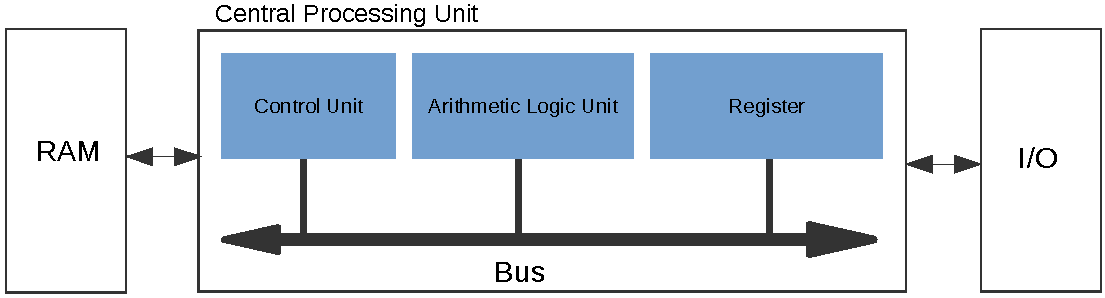
\includegraphics[width=1.0\textwidth]{images/cpu.pdf}
\caption{Central Processing Unit}
\label{fig:CPU}
\end{figure}

\section{Aufbau des Linux Betriebssystems}
% Monolithische Systeme 
% TRAP-Instruktion

Durch das Betriebssystem Minix, das von Andrew S. Tanenbaum für Ausbildungszwecke erstellt wurde, inspiriert, machte es sich Linus Torvalds zum Ziel, dieses vollwertige System neu zu schreiben. Im Jahr 1991 erschien die erste Linux Version 0.01\cite{ehses2011systemprogrammierung_chap2}. Heute ist es ein weit verbreitetes Betriebssystem, das für unterschiedlichen Anwendungszwecke wie für Desktops, Server, Smartphones und Embedded Systems eingesetzt wird.
\par
Die Aufgabe des Betriebssystemkerns, der meistens einfach nur Kernel genannt wird, ist es, eine Softwareschicht zwischen Hardware und Programm zu erstellen. Die Programme haben somit keinen direkten Zugriff auf die Hardware. Jedes Programm, das Informationen der Hardware benötigt, muss durch die Schicht des Kernels gehen. Die Kommunikationen zwischen Programm und Kernel werden Systemaufrufe (engl. Systemcalls) genannt. Die unterschiedlichen Systemaufrufe sind im POSIX standardisiert\cite{ehses2011systemprogrammierung_chap2}. Zusätzlich erstellt der Kernel eine Art Abkapselung eines Programms. Dadurch können mehrere Programme gleichzeitig laufen, ohne dass das eine Programm Zugriff auf das andere hat. Der Kernel verteilt die freien Ressourcen der CPU abwechslungsweise an die Programme. Dieses Verfahren heisst Multitasking und wurde seit den Anfängen unterstützt.
\par
Durch die zusätzliche Softwareschicht, die der Kernel bietet, müssen Programmierer ein Programm nicht für eine bestimmte Hardware schreiben, sondern für ein bestimmtes Betriebssystem. Dies ermöglicht eine höhere Portabilität eines Programms. Hardware wie Festplatten oder Netzwerkcontroller werden vom Kernel vereinheitlicht und dem Programm durch Systemaufrufe zur Verfügung gestellt.
\par

\begin{wrapfigure}{L}{0.49\textwidth}
\centering
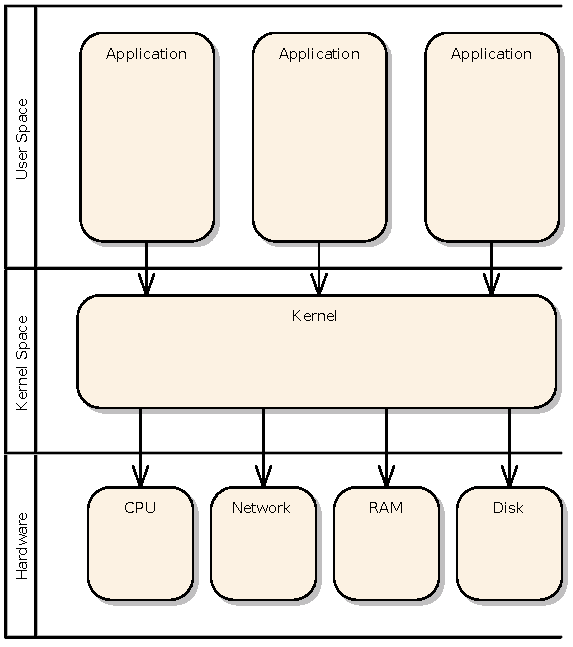
\includegraphics[scale=0.8]{images/kernel.pdf}
\caption{Linux Kernel}
\label{fig:kernel}
\end{wrapfigure}

Die \autoref{fig:kernel} zeigt, wie die unterschiedlichen Schichten miteinander kommunizieren. Eine Anwendung wird ausschliesslich im Benutzermodus (engl. User Space) ausgeführt. Durch Systemaufrufe werden Anfragen an den Kernel übermittelt. Dabei findet ein Kontextwechsel vom unprivilegierten in den privilegierten Modus statt. Der unprivilegierte Modus bezeichnet den Benutzermodus, in dem eine Applikation nur beschränkt über den Arbeitsspeicher verfügen kann und nur gewisse CPU-Befehlssätze ausgeführt werden können. Dies stellt sicher, dass eine Applikation gegenüber dem Rest des Systems abgekapselt betrieben wird und nicht darauf zugreifen kann. Nach dem Systemaufruf geht der Prozessor in den privilegierten Modus über und der Kernel trägt die Verantwortung, die Anfrage im Kernelmodus (engl. Kernel Space) zu verarbeiten. Der Kernelmodus weist im Gegensatz zum Benutzermodus keine Einschränkungen auf und hat deswegen auch Zugang zur Hardware und zum gesamten Arbeitsspeicher. Demzufolge dient der Kontextwechsel dazu, dass derjenige Programmcode, der nicht zum Kernel gehört, nur in einem unprivilegierten Modus ausgeführt werden kann.


\section{Unterschiede zwischen CISC- und RISC-CPUs\cite{todo}}

Die CPUs können, je nach dem wie ihre Befehlssatzarchitektur aufgebaut ist, in unterschiedliche Gruppen aufgeteilt werden. CISC-Prozessoren (Custom Instruction Set Computer) weisen im Vergleich zu RISC-Prozessoren (Reduced Instruction Set Computer) sehr komplexe und umfangreiche Befehlssätze auf.
\par
Im Jahr 1978 führte Intel mit dem 8086 Prozessor den x86-Befehlssatz ein. Dieser wurde zum Urvater moderner CISC-Prozessoren. Schon damals besass dieser Prozessor zirka 120 Befehlssätze. Im Verlauf der Jahre zeichneten sich die CISC-Prozessoren durch immer mehr und komplexere Befehlssätze aus. Dabei wurde stets darauf geachtet, dass die Architektur der neueren Modelle rückwärtskompatibel ausgestaltet ist, damit ältere Software auch ohne Anpassung auf neueren Prozessoren laufen kann. Die CISC-Architektur erlaubt es, komplexe Instruktionen in einem Befehlssatz zu schreiben. Dabei wird der Befehlssatz von der CPU dekodiert und in einem oder mehreren Taktzyklen ausgeführt. Die Komplexität der Befehlssätze geht so weit, dass sogar Hardwareschleifen möglich werden. Weiter kann ein Befehlssatz die Anweisung erhalten, Daten von einer Speicherzelle im RAM direkt zu einer anderen zu transferieren, ohne dabei auf ein Register angewiesen zu sein. Daher verfügen die meisten CISC-Prozessoren in der Regel über eine geringere Anzahl von Register als RISC-Prozessoren. Zusätzlich besitzen die gegenwärtigen CISC-Prozessoren sehr umfassende Steuerwerke, damit sie die immer komplexeren Befehlssätze dekodieren und in Instruktionen aufteilen können. Die Steuerwerke dieser Prozessoren bestehen normalerweise aus Hardware-Implementationen. Jedoch können sie innerhalb des Steuerwerks ebenso Microcode, also eine Software-Implementation, aufweisen.
\par
Bis Mitte der Achtziger war man der Meinung, dass durch komplexere Hardware und die damit verbundene höhere Anzahl an verfügbaren Befehlssätzen eine grössere Leistung erzielt werden kann. Der Trend zu immer mehr und vielfältigeren Befehlssätzen nahm aber ab. Dies hat zur Folge, dass heute einerseits kaum noch Programme in Assembler geschrieben und andererseits die gängigen Compiler so gebaut werden, dass sie nur noch etwa 20 Prozent der Befehlssätze benötigen. Dazu kommt, dass die komplexen Verarbeitungsstrukturen innerhalb eines CISC-Prozessors die Elementaroperationen verlangsamen.
\par
Patterson, David A. und Sequin, Carlo H. prägten zwar Ende der achtziger Jahre den Begriff "RISC" \cite{Patterson:1981:RIR:800052.801895}, jedoch existierten diese Art der Prozessoren mit einfacher Architektur bereits seit geraumer Zeit. Die Technik war noch nicht sehr ausgereift und die Prozessoren konnten nur eine begrenzte Anzahl an Instruktionen verarbeiten. RISC-Prozessoren zeichnen sich durch eine Load-and-Store-Architektur, eine höhere Menge an Universalregistern und die Begrenzung auf Elementarinstruktionen aus. Der Begriff "Load and Store" meint, dass Daten stets über Register geladen und gespeichert werden müssen. Demnach ist es bei dieser Architektur nicht möglich, die Daten von einer Speicherzelle im RAM zu einer andere zu transferieren, ohne sie zuerst in einem Register zwischenzuspeichern. Es benötigt bei diesem Vorgehen somit immer mindestens zwei Taktzyklen; den ersten zum Laden der Daten in ein Zwischenregister und den zweiten zum Abspeichern dieser in eine andere Speicherzelle. Aufgrund der grösseren Anzahl an Registern muss ein RISC-Prozessor bei der Ausführung von Instruktionen daher weniger auf den Speicher zurückgreifen als ein CISC-Prozessor.
\par
Die frühere klassische Trennung zwischen CISC- und RISC-Prozessoren wird immer wie kleiner. Die Entwicklung der CISC-Prozessoren hat sich stark an derjenigen von RISC-Prozessoren ausgerichtet, da sie intern praktisch mit einer RISC-Struktur und einer hochentwickelten Vorverarbeitungsstufe ausgestattet sind. Bereits der Pentium Pro war mit einem RISC-Kern ausgestattet und die von aussen ersichtliche x86-Schnittstelle war, so zu sagen, ein vorgeschalteter x86-Emulator.



%\section{Energy Storage in a Capacitor}
%Grundlage Technische Informatik Kap. Halbleitertechnik lesen!



\section{Relevanz für das Experiment}

Prozessoren sind als elektronische Schaltkreise realisiert. Die Schaltkreise werden durch die Halbleitertechnologie hergestellt. Die Millionen von witzigen Transistoren, die ein Prozessor beinhaltet, werden zu logischen Bausteinen verdrahtet.
\par
In dieser Arbeit ist die Funktionsweise der ALU relevant. Wir wissen, dass die ALU eine Reihe von Anweisungen erhält und somit jeden erdenklichen Algorithmus ausführen kann. Im Rahmen dieser Arbeit wird eine Methode entwickelt, um den Energieverbrauch einer einzelnen Anweisung der ALU messen können.





%Table 1.2. Double-precision VFP operations
%Instruction types	Issue latency
%DP MUL and MAC	2 cycle
%SP DIV, SQRT	14 cycles
%DP DIV, SQRT	28 cycles
%All other instructions	1 cycle


\chapter{Idee und Zielsetzung}


\chapter{Aufbau des Experiments}

In diesem Kapitel wird die Methode beschrieben, die in dieser Arbeit zur Messung der Energie eines Befehlssatz verwendend wird. Für das Verständnis wird auf die technische Elemente eingegangen, die für das Experiment nötig sind.
\section{Auswahl und Beschreibung der Messmethode}
\label{chap:auswahl_beschreibung_methode}

Während die CPU ein Programm ausführt, das aus einer Reihe von Befehlssätzen besteht, verbraucht sie unterschiedlich viel Strom. Die Idee der hier erstellten Messmethode ist es, ein Programm kontrolliert und mit präzis ausgewählten Befehlssätzen auf der CPU durchlaufen zu lassen. Das Programm in Form eines Benchmarks ist so konzipiert, dass ein bestimmter Befehlssatz millionenfach wiederholt wird. Dadurch wird der Stromverbrauch während der Ausführung über einen längeren Zeitraum konstant gehalten. Denn nur so ist eine aussagekräftige Messung möglich, da ein einzelner Befehlssatz so schnell durchläuft, dass er kaum messbar ist. Da die Ausführung der Befehlssätze wiederholt wird, muss die Messung durch die Anzahl der ausgeführten Wiederholungen geteilt werden.
\par
Die Strommessung erfolgt vom Leistungsverbrauch des ganzen Gerätes. Optimal wäre es, nur die Leistung der CPU zu messen. Dafür müsste aber die CPU vom Board ausgelötet und eine speziell dafür gebaute Messvorrichtung verwendet werden. Dazu kommt, dass nicht alle Datenblätter, welche die erforderliche Beschreibung und Belegung der Pins enthalten, für jedes Board oder für jeden Chip verfügbar sind. Deshalb wird ein SoC eingesetzt und die gesamte Leistung gemessen. SoC sind verfügbar auf kleinen Entwickler-Boards, die keine Lüfter, Laufwerke oder andere Verbraucher aufweisen, die hinsichtlich der Leistung störende Unregelmässigkeiten verursachen würden.



\begin{wrapfigure}{R}{0.6\textwidth}
\centering
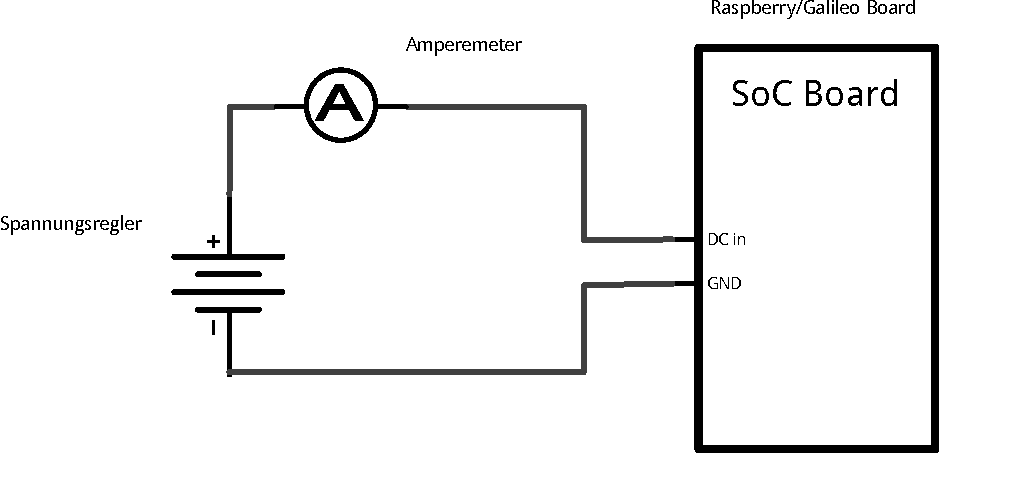
\includegraphics[scale=0.5]{images/schema.pdf}
\caption{Elektroschema für die Messung}
\label{fig:Elektroschema}
\end{wrapfigure}


Die für diese Arbeit verwendeten Boards werden im nächsten Kapitel im \autoref{beschreibung_hardware} beschrieben. Es wird davon ausgegangen, dass die Komponenten auf dem Board, abgesehen vom CPU selbst, während der Durchführung des Benchmarks vernachlässigbar kleine Leistungsschwankungen aufweisen. Die Messung erhält somit lediglich die Grundleistung der CPU, die vom Resultat abgezogen werden muss. Die Speisung erfolgt über einen Spannungsregler, der der Schaltung eine konstante Spannung liefert. Zwischen dem Spannungsregler und der Schaltung ist ein Amperemeter (Multimeter) zwischengeschaltet, der die Messung vornimmt. In der Abbildung \ref{fig:Elektroschema} ist das Elektroschema und die Platzierung des Amperemeters ersichtlich.
\par
Der eigentliche Kern des Benchmarks besteht aus gezielten und kurzen Assembler-Zeilen. Der Assemblercode bewirkt eine Schleife über einen zu testenden Befehlssatz. Damit das Ergebnis über einen längeren Zeitraum gemessen werden kann, wird der zu testende Befehlssatz einige Milliarden Mal  wiederholt. So wird ein Zeitraum von zirka zwei bis drei Minuten erzeugt, in welchem die Messung auf einem 800MHz CISC-Prozessor vorgenommen werden kann.
\par
Während dem Durchlaufen des Benchmarks darf die Ausführung nicht gestört werden. Jedes moderne Betriebssystem ist multitaskingfähig. Das bedeutet, dass das Betriebssystem eine Zeitscheibe besitzt und die Ressourcen der CPU abwechslungsweise an die Prozesse verteilt werden. Ein Benchmark darf also nicht als gewöhnlicher Prozess von einem Betriebssystem gestartet werden. Würde man das tun, hätte man keine Kontrolle, wann und wie viele Ressourcen der Benchmark schliesslich zugesprochen bekommt. Diese mangelnde Kontrolle würde das Messresultat verfälschen. Im Rahmen dieser Arbeit musste daher eine Methode erarbeitet werden, bei der der Benchmark während der Durchführung die vollen Ressourcen der CPU zugeteilt erhält und somit ein kontrollierter Ablauf garantiert ist.
\par
Die Ursprungsidee war es, direkt auf Baremetal zu arbeiten. Baremetal ist eine Ausdruck dafür, dass direkt auf der Hardware gearbeitet wird. Bei dieser Methode wird auf ein Betriebssystem verzichtet. Nach dem Bootprozess der Hardware wird ein Programm direkt gestartet und ausgeführt. An dieser Stelle wäre der Benchmark zum Zug gekommen. Eine speziell dafür präparierte Partition bootet die Hardware und führt den Benchmark aus.
\par
Für die Baremetal-Methode wurde ein funktionstüchtiger Prototyp erstellt. Es zeigten sich aber einige Nachteile. Auf komplexerer Hardware mit x86-Prozessoren ist der Boot-Vorgang um ein Vielfaches aufwendiger\cite{intel_boot_process}. Diese Prozessoren-Typen können nicht einfach beim Einschalten einen Programmcode ausführen. Es muss vorher eine lange Reihe von Abläufen in der Preboot Phase berücksichtigt und ausgeführt werden. Ein weiterer Nachteil der Baremetal-Methode ist die Überprüfung des Benchmarks. Die Gewährleistung, dass der Benchmark erwartungsgemäss funktioniert beziehungsweise überhaupt ausgeführt wird, benötigt ein Feedback nach aussen. Eine LED-Leuchte würde für dieses Feedback bereits ausreichen. Allerdings sind die GPIOs, die benötigt werden, um das LED zu steuern, je nach SoC sehr schwer anzusprechen, weil sie über einen PCI-Bus verbunden sind. Normalerweise stellt das Betriebssystem die nötigen C-Libraries zur Verfügung, um Komponenten, wie die GPIO, über einen PCI-Bus anzusteuern. Dieses fehlt hier jedoch gerade. Negativ wirkt sich zusätzlich die aufwendige Vorbereitung jedes einzelnen Tests aus. Für jeden Test muss eine Partition mit dem Benchmark erstellt und auf ein Medium kopiert werden. Damit die Messung erfolgen kann, muss dabei auch jedes Mal die Hardware neu gestartet werden. Unter diesen Umständen wird ein automatisierter Betrieb erheblich erschwert.
\par
Wegen der oben genannten Nachteile, wurde ein neues Konzept ausgearbeitet. Das neue Konzept arbeitet auf dem Betriebssystem Linux und bringt dadurch dessen Vorteile mit sich. Es muss sichergestellt werden, dass der Benchmark ohne Unterbrüche und abgeschirmt von anderen Prozessen durchgeführt wird. Um dies zu erreichen, wird der Benchmark anstatt im Benutzermodus (engl. User Space) im Kernelmodus (engl. Kernel Space) ausgeführt\cite{Mandl2010}. Der Programmcode, der innerhalb des Kernelmodus ausgeführt wird, muss als Kernelmodul kompiliert und im Kernel angemeldet werden. Schliesslich kann nur ein Interrupt den Code im Kernelmodul ausführen. Die genaue Beschreibung wird nachfolgend im \autoref{chap:benchmark_basis_interrupts} erläutert. Durch die Vornahme des Benchmarks im Kernelmodul werden alle Prozesse, die auf dem Betriebssystem parallel laufen, gestoppt und der Benchmark bekommt die vollen CPU-Ressourcen zugesprochen. In ein Kernelmodul können unterschiedliche Benchmarks gleichzeitig hinein kompiliert werden. Somit wird die Ausführung unterschiedlicher Tests vereinfacht. Dadurch wird eine spätere Automatisation ermöglicht, was zu einer Erleichterung der Messung beiträgt. 

 



 

\section{Beschreibung der Hardware}
\label{beschreibung_hardware}
\subsection{Intel Galileo Gen2}

\begin{wrapfigure}[14]{R}{0.6\textwidth}
\centering
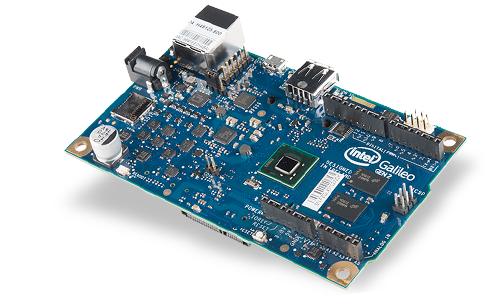
\includegraphics[scale=0.5]{images/iot_galileo.png}
\caption{Intel Galileo Gen2\cite{intel_galileo_image}}
\label{fig:Intel Galileo Gen2}
\end{wrapfigure}

Das Galileo Developer Board\cite{intel_datasheet_galileo} der zweiten Generation von
Intel ist ein SoC und besitzt einen Intel® Quark™ SoC X1000 Prozessor. Die Architektur des 32bit Prozessor basiert auf x86\cite{intel_datasheet} und somit ist das Galileo
Board eines der wenigen, auf denen ein CISC-Prozessor verbaut wurde. Die Hardware
besitzt keinen Videoausgang. Es ist also nur möglich, über eine RS232 Schnittstelle oder über Ethernet,
eine Verbindung zum System zu erstellen. Die GPIO Ein- und Ausgänge sind über den
PCI-Bus verbunden. Somit ist es sehr schwer, den GPIO ohne passenden Treiber oder
Softwareschicht anzusprechen. Im Vergleich sind die GPIO des RaspberryPI, das als zweites Board gewählt wurde,
direkt über eine Speicheradresse ansprechbar.
\par
Von Intel wird ein angepasstes Betriebssystem als fixfertiges Image angeboten. Dieses System basiert auf
der Linux Distribution Yocto. Es sind aber auch inoffizielle Debian Distributionen im
Internet erhältlich. Der Vorteil von Debian gegenüber der offiziellen Version, ist die
grössere Verbreitung und die damit verbundenen Hilfestellungen im Internet. Das Cross-Compiling eines Kernelmoduls scheint so einfacher als auf der Yocto-Distribution.


\subsection{RaspberryPi}


\begin{wrapfigure}[18]{R}{0.6\textwidth}
\centering
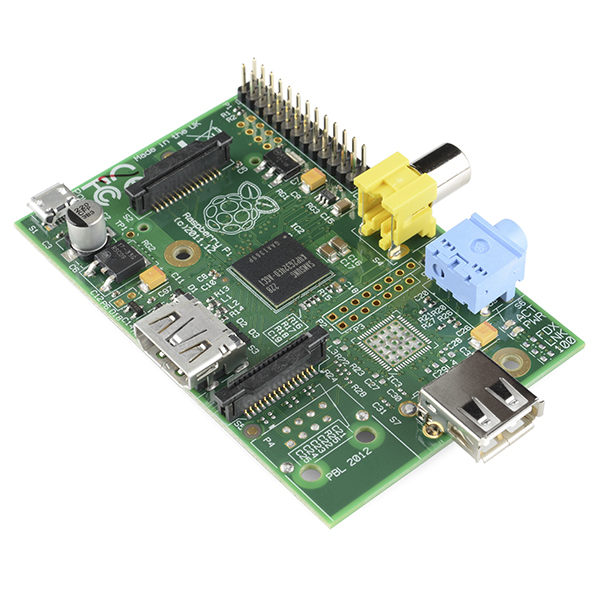
\includegraphics[scale=0.4]{images/raspberry-pi-2.png}
\caption{Raspberry Pi 1 A\cite{raspberry_image}}
\label{fig:Raspberry Pi 1 A}
\end{wrapfigure}


Als zweites Experimentier-Board wird das Raspberry Pi Model B\cite{raspberry_foundation} verwendet. Das Board wird von der Raspberry Pi Foundation betrieben. Das Modell besitzt einen Broadcom BCM2835\cite{broadcom_datasheet} Chip. Der darin verbaute Prozessor wurde von der Firma ARM unter dem Namen ARM1176JZFS\cite{arm_datasheet} (ARM11) spezifiziert. Die Software muss für die Architektur ARMv6 kompiliert werden. Im Gegensatz zum Galileo Board von Intel ist der Prozessor ein RISC-CPU. Beide Boards haben eine 32bit Adressierung.
\par
Eine Remote-Verbindung lässt sich über eine serielle Schnittstelle oder über Ethernet realisieren. Durch das Vorhandensein eines Videoausgangs und eines USB-Anschlusses würde sich das Raspberry Pi auch direkt über Monitor und Tastatur bedienen lassen. Die GPIOs sind direkt über die Speicheradressierung ansprechbar. Somit wäre eine Erweiterung des Benchmarks, der in Assembler geschrieben ist, durchaus denkbar. So könnten auf einfache Weise weitere Messungen über die GPIO erfolgen. Das offizielle Betriebssystem der Foundation ist ein Debian basiertes OS mit dem Name Raspbian. Zusätzlich werden als Third-Party Produkte weitere unterschiedliche Betriebssysteme zur Verfügung gestellt. 













\section{Benchmark auf Basis von Interrupts}
\label{chap:benchmark_basis_interrupts}

% A system call is a request in a Unix-like operating
% system made via a software interrupt by 
% Found on http://www.linfo.org/software_interrupt.html


Der Aufbau der Messmethode basiert auf Softwareinterrupts. Dafür wurde ein eigenes Kernel\-modul erstellt, das den Benchmark beinhaltet und auf Verlangen ausführt.
\par
Ein Interrupt zwingt den Linux Kernel, vom Benutzermodus in den Kernelmodus zu wechseln\cite{Mandl2010_3}. Beim Wechsel werden alle laufenden Prozesse zwischengespeichert und angehalten. Anschliessend wird eine Interrupt-Service-Routine (ISR) aufgerufen. Genau diese Eigenschaft wird für den Aufbau der Messmethode verwendet. Denn während der Ausführung der ISR sind alle Prozesse angehalten und können den Benchmark, der sich in der ISR befindet, nicht unterbrechen. Somit wird sichergestellt, dass nur der Benchmark ausgeführt wird und dieser die vollen Ressourcen der CPU bekommt, bis er abgeschlossen ist.
\par

\begin{wrapfigure}{l!}{0.5\textwidth}
\centering
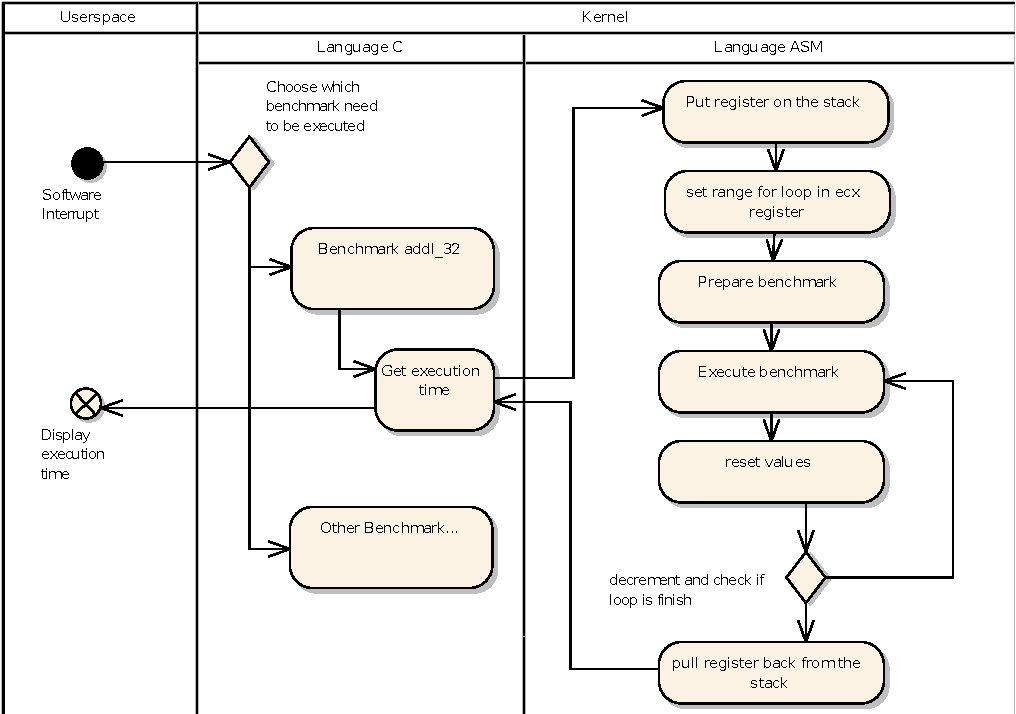
\includegraphics[scale=0.45]{images/interrupt_ea.pdf}
\caption{Interrupt}
\label{fig:Interrupt}
\end{wrapfigure}

Interrupts sind dafür gemacht, sofort verarbeitet zu werden. Ein kleines Beispiel soll dies veranschaulichen. Der Benutzer eines Computers drückt eine Taste auf der Tastatur. Dadurch produziert er ein Hardware-Interrupt. Der aktuelle Prozess wird gespeichert und angehalten. Der Kernel stellt über eine Vektor-Tabelle fest, um welchen Interrupt es sich handelt und führt die passende ISR aus, die zur Verarbeitung der gedrückten Tasten dient. Die ISR besteht aus einem sehr kurzem Programmcode (Microcode). In diesem Fall speichert der Programmcode die gedrückte Taste im RAM und gibt die Ressourcen wieder frei. Der letzte Prozess wird danach, falls er nicht bereits beendet war, weitergeführt. Die Interrupts sind nötig, um die Daten im Zeitpunkt des Geschehens zu verarbeiten.
\par

\autoref{fig:Interrupt} stellt die unterschiedlichen Interrupts und den Ablauf nach einem eingehenden Interrupt dar. Die Hardware-Interrupts\footnote{Je nach Literatur, Sprache oder Betriebssystem werden unterschiedliche Fachausdrücke verwendet. Der Kontext bleibt aber derselbe.} wurden bereits oben beschrieben. Die "Exception / Trap" sind Interrupts, die die CPU selber produziert. Ein Beispiel für ein solches Interrupt ist "Divisions by Zero". Dabei probiert man, eine Zahl durch Null zu teilen. Die Messmethode in dieser Arbeit stützt sich auf Software-Interrupts. Software-Interrupts werden als Systemcall bezeichnet, die häufig verwendet werden, um durch einen Kontextwechsel eine Aufgabe dem Kernel zu übergeben. Beim Kontextwechsel wird vom unprivilegierten Ring (Benutzermodus) in den privilegierten Ring (Kernelmodus) gewechselt. Dadurch kann auf Befehlssätze und Speicheradressen zugegriffen werden, was im Benutzermodus nicht möglich wäre, ohne unsicheren Code ausführen zu müssen. Systemcalls werden als ISR im selben Kontext ausgeführt wie Interrupts.




\section{Starten des Benchmarks über procfs}

Der Benchmark wurde in Form eines Kernelmoduls für ein Linux Betriebssystem gebaut. Das Kernelmodul registriert für jeden Benchmark ein Pseudofile, das unter der Verzeichnisstruktur \texttt{/proc/benchmark/} abrufbar ist.
\par
Das \texttt{procfs} oder \texttt{proc filesystem} genannte Filesystem erstellt eine Schnittstelle zwischen dem Benutzermodus und dem Kernelmodus. Es ist ein virtuelles Filesystem, das unter der Verzeichnisstruktur \texttt{/proc} gemountet wird\cite{mauerer2010professional}. Die Dateien, die sich darin befinden, sind Pseudofiles. Sie sind virtuell, weil sie nicht physisch existieren und somit auch nicht auf ein Medium gespeichert werden können. Beim Schreiben beziehungsweise Lesen der Pseudofiles werden die Informationen dem Kernel weitergegeben, verarbeitet und die Informationen werden zum Lesen im Benutzermodus bereitgestellt. Weil das Verhalten der Schnittstelle den Eigenschaften einer Datei entspricht, können für die Lese- und Schreiboperationen die Linux-Standardwerkzeuge verwendet werden.

\lstset{language=bash}
\begin{minipage}{\linewidth}
\begin{lstlisting}[label={list:read_procfs},caption={Lesen im procfs}]
sriolo@desktop ~ $ cat /proc/uptime 
571433.06 1229766.89
\end{lstlisting}
\begin{lstlisting}[label={list:write_procfs},caption={Schreiben im procfs}]
sriolo@desktop ~ $ echo 1 > /proc/sys/net/ipv4/conf/default/forwarding
\end{lstlisting}
\end{minipage}


Im ersten Beispiel \autoref{list:read_procfs} wird aus der Datei \texttt{uptime} gelesen. Dabei wird durch einen Systemcall die Betriebszeit berechnet und zurückgegeben. Das folgende, zweite Beispiel \autoref{list:write_procfs} zeigt, wie in einer Datei geschrieben werden kann. Dabei wird dem Kernel mitgeteilt, dass er das IP-Forwarding einschalten soll. Einen ähnlichen Aufbau hat das \texttt{sys filesystem}. Die Kommunikation ist dabei schwieriger, weil das Design für Menschen nicht lesbar ist, sondern lediglich für Programme im Benutzermodus. Im Gegensatz dazu kann das \texttt{procfs} mit den Standard-Werkzeugen im ASCII-Format gelesen und geschrieben werden.
\par
Das \texttt{procfs} ist an dieser Stelle wichtig, weil der Benchmark im Kernelmodus laufen muss. Durch den Befehl \texttt{cat} auf die entsprechende Datei des Benchmarks startet im Kernelmodus der Ablauf für die Messung und gibt die verwendete Zeit als Ausgabe an. Das folgende Beispiel in der \autoref{list:start_benchmark} veranschaulicht, wie der Benchmark gestartet und die CPU durch eine Addieroperation ausgelastet wird.

\lstset{language=bash}
\begin{minipage}{\linewidth}
\begin{lstlisting}[label={list:start_benchmark},caption={Starten des Benchmarks}]
root@galileo ~ $ cat /proc/benchmark/addl_32
321
\end{lstlisting}
\end{minipage}


\section{Aufbau der Software für die Messung}


\subsection{Grundaufbau und Ablauf eines Benchmarks}
Der Grundbau der Software wurde mit der Programmiersprache C geschrieben. Der Kern des Benchmarks besteht aus wenigen Assembler-Befehlssätzen. Das Kernelmodul beinhaltet alle für diese Arbeit relevanten Benchmarks. Die \autoref{fig:Benchmark} stellt den Ablauf des Programms dar.

\begin{figure}[H]
\centering
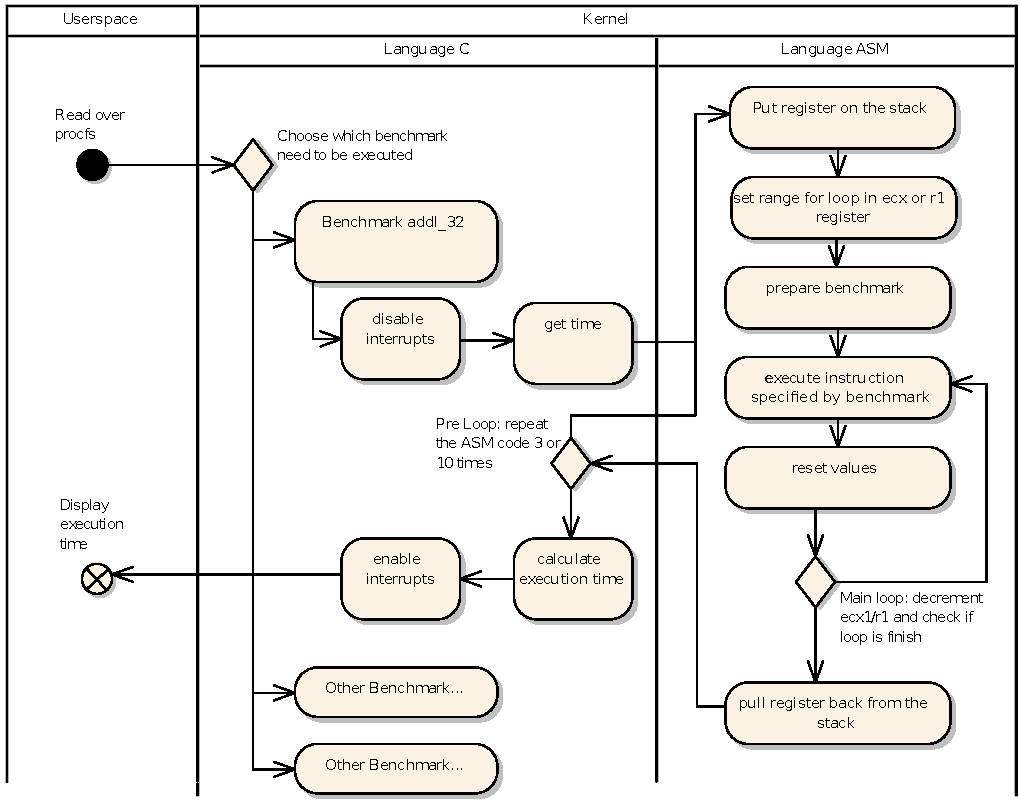
\includegraphics[width=1.0\textwidth]{images/benchmark_ea.pdf}
\caption{Benchmark}
\label{fig:Benchmark}
\end{figure}


Durch einen Systemcall, der über das \texttt{procfs} ausgelöst wird, wird der Benchmark gestartet. Da sich in der Software mehrere Benchmarks befinden, muss zuerst einer dieser Benchmarks ermittelt werden. An dieser Stelle werden durch die Funktion \texttt{local\_irq\_save} alle weiteren Interrupts geblockt. Die Startzeit wird eruiert und zwischengespeichert. Das Programm wechselt zum eigentlichen Benchmark, der in Assembler geschrieben ist. Ist der Assembler-Teil abgearbeitet, wird die Zeit errechnet, die zur Durchführung des Benchmarks verwendet worden ist. Durch den Aufruf der Funktion \texttt{local\_irq\_restore} wird die Blockierung von weiteren Interrupts wieder aufgehoben. Als letztes wird die vom Benchmark aufgewendete Zeit in den Systemcall zurückgeliefert.
\par
Die Grösse der Schleife, die in Assembler geschrieben worden ist, ist auf die Anzahl ihrer möglichen Wiederholungen beschränkt. Beide Boards haben eine 32bit-Architektur. Die maximale Anzahl der Durchläufe kann somit die Wortbreite von 32bit grundsätzlich nicht übersteigen. Damit die Messung eines Benchmarks dennoch über einen längeren Zeitraum gemessen werden kann, wird ein einfacher Trick angewendet. Um den Assembler-Code wird eine Vorschleife gelegt. Diese Vorschleife verlängert die Ausführung des Benchmarks um das drei- bis zehnfache. Die genaue Anzahl der Durchgänge pro Board ist aus \autoref{fig:benchmark_loop_size} ersichtlich. Die Auswirkungen der Vorschleife auf das Messresultat sind gering, da die Vorschleife um ein x-faches kleiner ist als die Endschleife. Demzufolge beeinflusst sie das Ergebnis kaum und ist dementsprechend vernachlässigbar.

\begin{figure}[H]
\center
\begin{tabular}{ |l|l|l|l| }
\hline
Board & Vorschleife (C) & Endschleife (Assembler) & Total \\ \hhline{|=|=|=|=|}
Galileo & 3 & 2147483648 & $\approx$6.4 Mrd.  \\ \hline
Raspberry & 10 & 2147483648 & $\approx$21.4 Mrd. \\ \hline
\end{tabular}
\caption{Anzahl Durchläufe eines zu testenden Befehlssatzes}
\label{fig:benchmark_loop_size}
\end{figure}



\begin{minipage}{\linewidth}
\lstset{language=[x64]Assembler}
\begin{lstlisting}[label={list:asm_benchmark},caption={Benchmark in Assembler}]
benchmark_imull_zero:
  stmfd    sp!, {r0-r5}
  ldr r1, = 2147483648
  ldr r3, = 0x0
  ldr r4, = 0x0
loop_benchmark_imull_zero:
  mul r5, r3, r4
  sub r1, r1, #1
  cmp r1, #0
  bge loop_benchmark_imull_zero
  ldmfd    sp!, {r0-r5}
  bx  lr
\end{lstlisting}
\end{minipage}


In der \autoref{list:asm_benchmark} ist der Assemblercode aufgeführt, der die CPU über einen längeren Zeitraum mit der Rechenoperation $0*0$ stresst. Die \autoref{list:asm_benchmark} dient als Beispiel für die Grundstruktur eines Benchmarks. Auf dieser basieren dann die unterschiedlichen Benchmarks, die je einen Befehlssatz beinhalten, der mit den anderen verglichen werden kann. Der Prozessor startet bei Zeile 1 und im nächsten Schritt werden alle Register \texttt{r1} bis \texttt{r5} im RAM auf einen Stack gelegt. Das Register \texttt{r1} wird mit $2^{31}$ gefüllt. Dieses dient dazu, später eine Schlaufe zu erzeugen. In Zeile 4 und 5 wird der Benchmark auf die Rechenoperation vorbereitet, wobei \texttt{r3} und \texttt{r4} auf null gesetzt werden. Der Prozessor wechselt nun zur wichtigsten Zeile, der Nummer 7. An dieser Stelle befindet sich die Multiplikationsoperation, die eine Veränderung des Energieverbrauchs erzeugt und diesen misst. Nach der Abarbeitung wird der Index im Register \texttt{r1} um eins dekrementiert. Anschliessend wird überprüft, ob der Index bereits null erreicht hat. Falls der Index noch nicht auf null ist, wird ein Programmsprung auf Zeile 7 erzeugt und die Schleife noch einmal wiederholt. Falls der Index null erreicht hat, wird der Programmsprung nicht erzeugt und dies führt zum Austritt aus der Schleife. Die Register \texttt{r1} bis \texttt{r5}, die am Anfang auf den Stack gelegt wurden, werden aus dem RAM geholt und wiederhergestellt. Damit ist das Assemblerprogramm zu Ende.
\par
In der \autoref{list:asm_benchmark} ist erkennbar, dass mehrere Befehlssätze erforderlich sind, um eine Schleife zu erstellen. Obwohl nur die Zeile 7 für den Benchmark relevant ist, müssen die Zeilen 8, 9 sowie 10 zwangsläufig programmiert werden und verfälschen das Messresultat. Damit ein aussagekräftiger Vergleich zwischen unterschiedlichen Benchmarks erstellt werden kann, muss die Grundstruktur daher immer gleich sein. Somit ist die Messung zwar nicht korrekt, da es sich jedoch immer um den gleichen Fehler handelt, können Vergleiche zwischen den Benchmarks gezogen werden.


\subsection{Kompilation und Programmstruktur}

\begin{wrapfigure}{!}{0.7\textwidth}
\centering
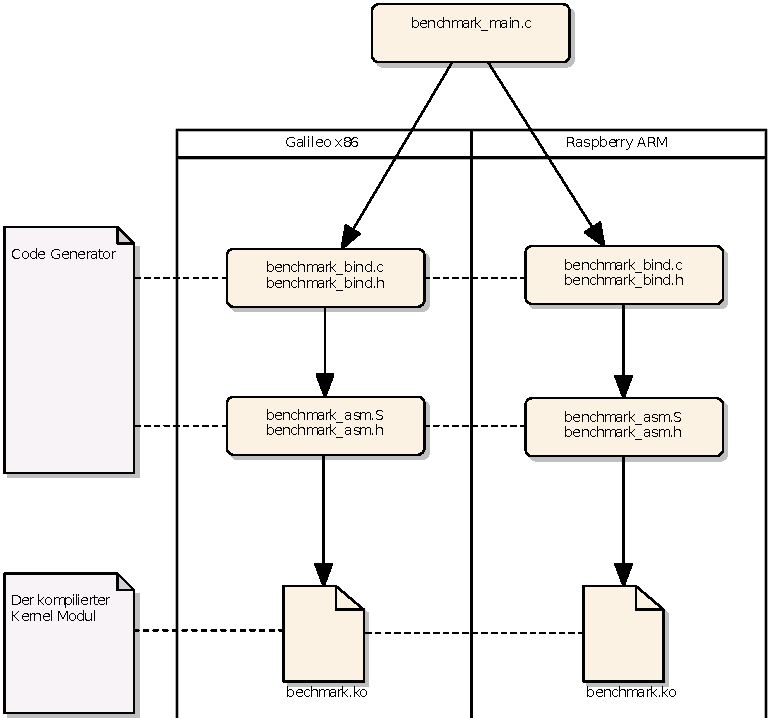
\includegraphics[scale=0.7]{images/filestructure.pdf}
\caption{Dateistruktur}
\label{fig:filestructure}
\end{wrapfigure}


Da die Grundstruktur des Benchmarks für jede Messung immer gleich ist, wurde ein Code-Generator in Python geschrieben. Dieser erstellt für jeden Benchmark automatisch die Grundstruktur und übernimmt den Inhalt aus einer Konfigurationsdatei. Der Code-Generator wird vor dem Kompilieren automatisch gestartet. Die Dateien werden an den richtigen Ort geschrieben, damit sie der GCC kompilieren und anschliessend mit dem Kernelmodul verlinken kann. Die Grundstruktur des Kernelmoduls liegt in der Datei \texttt{benchmark\_main.c}. Die Datei \texttt{benchmark\_bind.c} sorgt für den Übergang von C in Assemblercode, der sich in der Datei \texttt{benchmark\_asm.S} befindet.
\par
Der Kompiliervorgang dauert auf einem SoC zu lange, weil der Prozessor zu schwach ist. Deshalb wurde das Kernelmodul für die SoCs auf eine leistungstarke Maschine kompiliert. Wenn Sourcecode auf einer Maschine für eine andere Maschine kompiliert wird, heisst dieser Vorgang cross-kompilieren. Wird nun während dieses Vorgangs ein Kernelmodul kompiliert, muss der Kompiler die Headerfiles des Kernels, in den das Kernelmodul später eingefügt wird, kennen. Zusätzlich enthält nicht jede Linux-Distribution Headerfiles. Dies gilt insbesondere auch für das RaspberryPi. Deshalb wird für dieses ein modifizierter GCC benötigt. Dieser steht auf der offiziellen Seite von Raspberry zum Download bereit. Vor der Kompilation müssen also die passenden Kernels auf der leistungsstarke Maschine erbaut und der modifizierte GCC für das RaspberryPI installiert werden. Nur so ist eine erfolgreiche Kompilation durchführbar. Die technische Dokumentation findet sich im Wiki meines Projektes zur Thesis unter \url{https://github.com/codeix/thesis_ffhs_2016/wiki}. Auf der gleichen Plattform stehen auch alle erforderlichen Dateien zur Nachvollziehbarkeit des Experiments zum Download bereit (ca. 800MB). Nach dem fehlerfreien Kompilieren des Kernelmoduls kann dieses auf das Board kopiert und mit dem Befehl \texttt{insmod} in den Kernel geladen werden.



\section{Automatisierung der Messung}
\label{sec:automatisierung}

Die Automatisierung der Messungen ist nicht ein notwendiges Element. Jeder Benchmark kann von Hand ausgeführt werden und parallel die Messung vorgenommen werden. Die Automatisierung soll aber helfen eine grössere Menge an Tests effizient vornehmen zu können. Ein sehr Wichtiger bestand der Automatisierung ist die Wiederholung von Tests. So kann eine Aussage gemacht werden, dass die Messung auch durch eine Wiederholung das selbe Resultat liefert und nicht von Störfaktoren beeinträchtigt wurde. Auch vereinfacht die Automatisierung die Anpassung von Test und erspart viel Zeit nachdem eine Ergänzung vorgenommen werden musste. Der Output erfolgt in Form von CSV-Dateien, die später in Diagramme dargestellt werden können.
\par
Für die Automatisierung wurde ein Python-Programm geschrieben, der auf ein zusätzlichen Computer ausgeführt wird. Der Computer ist mit einem Amperemeter (Multimeter) verbunden und hat über eine Remoteshell Zugang zum Board. Die Benchmarks in Form eines Kernelmoduls sind bereits auf dem Board installiert und können über das \texttt{procfs} gestartet werden. Die folgende List zeigt den Ablauf der automatisierte Durchführung der Messung:


\begin{enumerate}
\item Anhand der selben Konfiguration-Dateien, die beim generieren der Benchmark-Source-Code verwendet wurden, wird zufällig die Reihenfolge für die Durchführung der Benchmark bestimmt. Dabei wird jeder Benchmark drei mal in dieser Reihenfolge hinzugefügt.
\item Der Reihenfolge nach wird ein Benchmark auf ein ausgewähltes Board ausgeführt. Die Durchführung dauert in der Regel 120 Sekunden. Die genau Durchführungszeit wird aber im Benchmark selber gemessen.
\item Parallel zur Durchführung des Benchmark wird im ungefähren Sekundentakt\footnote{Das Messgerät sendet die Daten als RS-323-Protokoll über eine USB-Schnittstelle. Mit dem hier verwendeten Messgerät hat man keine Einfluss über die Sendeperiode.} der Strom gemessen. Dieser erfolgt über eine USB-Schnittstelle zum Amperemeter (Multimeter). Die Daten werden zwischen gespeichert, bis sie zum Schluss in einer CSV-Datei geschrieben werden können.
\item Der Benchmark hat nach Durchführung, die verwendete Zeit als Rückgabewert. Dieser Wert entspricht der sehr genau Durchführungszeit und wird ebenfalls Zwischengespeichert damit sie zum Schluss in einer Datei gespeichert werden kann.
\item Nach der Durchführung wird eine Pause von einer Minute eingelegt. Diese Pause ist wichtig damit alle Benchmarks gleich behandelt werden. Durch die Durchführung eines Benchmarks kann die Temperatur des Board erheblich ansteigen. Werden die Benchmarks ohne Zwischenpause der reihe nach ausgeführt, kann es zu verzerrte Messwerte führen.
\item Die Schritte werden Wiederholt bis alle Benchmarks drei Mal durchlaufen worden sind. Sind alle Benchmarks abgearbeitet werden die Daten, die Zwischengespeichert worden sind, strukturiert und in Dateien geschrieben.
\end{enumerate}

\chapter{Resultate}

\section{Beschreibung der Daten}

Die Daten wurden automatisiert, wie im \autoref{sec:automatisierung} beschrieben, aufgezeichnet und als Diagramme dargestellt. Die Resultate befinden sich im Anhang dieser Arbeit. Die Beschreibung zu den Daten sind wie folgt zu interpretieren:

\begin{description}
\item[Titel]
Der Titel entspricht dem Benchmark das ausgeführt wurde. Der Name vordem Unterstrich ist auch der Befehlssatz, dass für den Benchmark verwendet worden ist. Wenn nach dem Unterstrich eine Zahl steht, definiert sie wie viele Bit das 32Bit-Register ausfüllt. Folglich steht z.B. für die Zahl 8 für die hexadezimale Zahl 0x000000FF.
\item[Beschreibung]
Jeder Benchmark besitzt eine Beschreibung die unmittelbar nach dem Titel steht.
\texttt{CSV-Datei} Die in kursiv geschriebene Datei definiert welche Daten für die Diagramme verwendet worden sind. Die Daten wurden im CSV-gespeichert und sind sind unter folgende URL zu finden: \url{https://github.com/codeix/thesis_ffhs_2016/tree/master/results}. Die Dateien sind entsprechend dem verwendeten Board in die Unterverzeichnisse \texttt{galileodata} und \texttt{raspberrydata} unterteilt. 
\item[Diagramme]
Die Daten sind als Liniendiagramm dargestellt. Jeder Benchmark wurde drei Mal ausgeführt, deswegen werden die Daten in drei Säulen dargestellt. Die Achsen wurden so ausgewählt, dass sie den Ausschnitt der relevanten Daten aufzeigen und möglichst viel Platz sparen.
\item[Durchschnitt und Median]
In der selbe Säule des Diagramm sind die Werte des Durchschnitt und Median aufgeführt. Beschriftet sind sie auf Englisch mit \texttt{Average} und \texttt{Median}.
\item[Durchlaufzeit]
Mit \texttt{Exec time} ist die Durchlaufzeit des Benchmark in Millisekunden aufgeführt. Da dieser Wert direkt vom Benchmark stammt, ist er genauer als der im Diagramm (Die Amperemessung wurde mit einer separater Uhr im Multimeter aufgezeichnet).
\item[Reihenfolge] Die Reihenfolge die mit \texttt{Exec order} bezeichnet ist, bestimmt in welche Folge die Daten aufgenommen worden sind. Die Benchmarks wurden nach einer Zufälliger Reihenfolge ausgeführt.

\end{description}



\section{Prüfung der Daten}


\section{Auswertung der Resultate}

\begin{filecontents}{dataset}
Pos	Name	Bench1	Bench2	Bench3	time1	time2	time3	medbench	medtime	energymWh	power
1	nop	431.9	432	432	129147	129147	129147	432	129.147	98.565	2.74752
2	nop\_nop	430.2	430.4	430.3	145291	145291	145291	430.3	145.291	110.45	2.736708
3	nop\_nop\_nop	431.1	431.1	431.1	161435	161434	161434	431.1	161.434	122.95	2.741796
4	addl\_0	431.4	431.8	431.5	145292	145291	145291	431.5	145.291	110.758	2.74434
5	addl\_32	435.3	435.2	435.5	145291	145291	145291	435.3	145.291	111.733	2.768508
6	subl\_0	431.4	432.1	431.4	145291	145291	145292	431.6	145.291	110.783	2.744976
7	subl\_32	435	435.2	435.3	145291	145291	145291	435.2	145.291	111.707	2.767872
8	shr\_0	432.8	432.8	433.5	177578	177579	177579	432.9	177.579	135.811	2.753244
9	shr\_32	432.7	432.6	432.9	177578	177578	177578	432.7	177.578	135.747	2.751972
10	shl\_0	433.1	432.9	432.9	177579	177579	177579	432.9	177.579	135.811	2.753244
11	shl\_32	432.7	432.9	433.2	177578	177578	177578	432.9	177.578	135.81	2.753244
12	imull\_0	427.9	427.3	427.4	226008	226008	226008	427.4	226.008	170.653	2.718264
13	imull\_32	429.7	429.5	429.9	226008	226008	226008	429.7	226.008	171.571	2.732892
14	inc\_8	436.4	435.6	435.7	145292	145291	145291	435.9	145.291	111.887	2.772324
15	dec\_8	433.9	434.4	434.6	161434	161434	161434	434.4	161.434	123.891	2.762784
16	and\_0	434.7	435.2	435.1	145292	145291	145291	435	145.291	111.656	2.7666
17	and\_32	428.6	429.7	430.6	145291	145291	145292	429.7	145.291	110.296	2.732892
18	or\_0	436	435.3	434.9	145291	145291	145291	435.35	145.291	111.746	2.768826
19	or\_32	429.8	431.2	431.4	145291	145291	145291	431.1	145.291	110.655	2.741796
20	xor\_0	432.5	431.5	431.5	145291	145292	145292	431.6	145.292	110.784	2.744976
21	xor\_32	434.2	435	435	145291	145292	145291	434.7	145.291	111.579	2.764692
\end{filecontents}



\begin{figure}[h] 
    \centering
    \begin{tikzpicture} 
        \begin{axis}[
            ybar,
            scale only axis,
            xlabel= Benchmarks,
            width = 0.85\textwidth,
            height = 0.25\textheight,
            y axis line style=blau_2b!100!black,
            ylabel= Leistungsvbrauch in W,
            % height = 80mm,
            ymin = 2.688264,
            ymax = 2.801052,
            xmin = 0,
            xmax = 22,
            bar width = 2mm,
            axis x line* = bottom,
            axis y line* = left,
            xticklabel style={rotate=90},
            xticklabels from table = {dataset}{Name},
            xtick = {1,...,21},
            bar shift = -1mm,
            y tick label style = {/pgf/number format/use comma},
            legend style = {at={(0.5, 1.025)}, anchor = south east, legend columns = -1, draw=none, area legend},
            area legend,
            extra y ticks ={2.688264},
            extra y tick style = {grid=none, yticklabel style={yshift=2.5mm, xshift=1.9mm, rotate=0, inner sep=.5pt}},
            extra y tick labels = {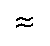
\includegraphics{almost_equals.eps}}
            ]
            \addplot+[mark=none, fill=blau_2a, draw = blau_2b] table[x=Pos, y=power, fill=red] {dataset};
            \legend{Leistungsverbrauch}
        \end{axis} 
        \begin{axis}[
            ybar,
            scale only axis,
            width = 0.85\textwidth,
            height = 0.25\textheight,
            y axis line style=gruen_4b!100!black,
            axis y line* = right,
            axis x line = none,
            ylabel = Durchlaufszeit in s,
            % height = 80mm,
            xmin = 0,
            xmax = 22,
            ymin = 0,
            xticklabel style={rotate=90},
            xticklabels from table = {dataset}{Name},
            xtick = {1,...,21},
            ymax = 246.008,
            ymin = 109.147,
            bar width = 2mm,
            bar shift = 1mm,
            legend style = {at={(0.5, 1.025)}, anchor = south west, legend columns = -1, draw=none, area legend},
            area legend,
            extra y ticks ={109.147},
            extra y tick style = {grid=none, yticklabel style={yshift=2.5mm, xshift=-1.6mm, rotate=0, inner sep=.5pt}},
            extra y tick labels = {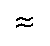
\includegraphics{almost_equals.eps}},
            ]
            \addplot+[mark=none,  fill=gruen_4a, draw = gruen_4b,] table[x=Pos, y=medtime] {dataset};
            \legend{Durchlaufszeit}
        \end{axis}
    \end{tikzpicture}
    \caption{Ausführung aller Benchmarks auf dem Galileo Board}
    \label{fig:benchmarks_galileo}
\end{figure}
























\chapter{Fazit}
\section{Diskussion}
%Vergleich mit ähnliche Papers (z.B. Energiemessung durch thermische Kamera)
Das Resultat in Sätze gefasst



\begin{appendix}


\chapter*{Selbständigkeitserklärung}
\addcontentsline{toc}{chapter}{Selbständigkeitserklärung}

Ich erkläre hiermit, dass ich diese Thesis selbständig verfasst 
und keine andern als die angegebenen Quellen benutzt habe. 
Alle Stellen, die wörtlich oder sinngemäss aus Quellen entnommen wurden, 
habe ich als solche kenntlich gemacht. Ich versichere zudem, dass ich bisher 
noch keine wissenschaftliche Arbeit mit gleichem oder ähnlichem Inhalt an der 
Fernfachhochschule Schweiz oder an einer anderen Hochschule eingereicht habe. 
Mir ist bekannt, dass andernfalls die Fernfachhochschule Schweiz zum Entzug 
des aufgrund dieser Thesis verliehenen Titels berechtigt ist.

\vspace{4cm}
\noindent
\hrule \ \\[-0.5ex]
Ort, Datum, Unterschrift
\end{appendix}




%\begin{thebibliography}{1}
%\end{thebibliography}
\bibliography{thesis_bibliography}
\bibliographystyle{gerplain}
\listoffigures



\end{document}


